\section{Efficient Semantic Parsing}
\label{sec:parsing}
In this section we explain our algorithms and heuristics for efficient semantic
parsing with as little ambiguity as possible, and reducing time complexity
of our parsing strategies.

\subsection{Syntactic-Semantic Parsing}
Using a naïve strategy of type checking on syntax trees yields an exponential
algorithm.
To avoid that, we extend the grammar system used to do the syntactic part of
the parsing to include semantic combination of words.
In this section, we will take the example of a CFG since it suffices to create
our typing combinators,
In Figure \ref{fig:combination-cfg}, we explicit a grammar of combination
modes, based on \cite{bumfordEffectdrivenInterpretationFunctors2025} as it
simplifies the rewriting of our typing judgements in a CFG.

\begin{figure}
	{\centering
\setlength{\columnsep}{-1.5cm}
\begin{multicols}{2}
	\def\arraystretch{1.2}
	\begin{mgrammar}
		\gskip
		\firstrule{>, b}{\left(a\to b\right), a}{}
		\firstrule{<, b}{a, \left(a \to b\right)}{}
		\firstrule{\wedge, a \to \t}{\left(a \to \t\right), \left(a \to \t\right)}{}
		\firstrule{\vee, a \to \t}{\left(a \to \t\right), \left(a \to \t\right)}{}
		\gskip
		\firstrule{\combJ_{\f{F}}\  \f{F}\tau}{\f{F}\f{F}\tau}{}
		\lfrule{\combDN_{\f{C}}\  \tau}{\f{C}_{\tau}\tau}{}
	\end{mgrammar}

	\def\arraystretch{1.3}
	\begin{mgrammar}
		\firstrule{\combML_{\f{F}} \left(\alpha, \beta\right)}{\f{F}\alpha, \beta}{}
		\firstrule{\combMR_{\f{F}} \left(\alpha, \beta\right)}{\alpha, \f{F}\beta}{}
		\firstrule{\combA_{\f{F}} \left(\alpha, \beta\right)}{\f{F}\alpha, \f{F}\beta}{}
		\firstrule{\combUR_{\f{F}} \left(\alpha \to \alpha', \beta\right)}{\f{F}\alpha\to \alpha', \beta}{}
		\firstrule{\combUL_{\f{F}} \left(\alpha, \beta\to \beta'\right)}{\alpha, \f{F}\beta \to \beta'}{}
		\firstrule{\combC_{\f{L}\f{R}} \left(\f{L} \alpha, \f{R}\beta\right)}{\left(\alpha, \beta\right)}{}
		\firstrule{\combER_{\f{R}} \left(\f{R}\left(\alpha \to \alpha'\right), \beta\right)}{\alpha\to \f{R}\alpha', \beta}{}
		\lfrule{\combEL_{\f{R}} \left(\alpha, \f{R}\left(\beta \to \beta'\right)\right)}{\alpha, \beta\to \f{R}\beta'}{}
	\end{mgrammar}
\end{multicols}
}

	\caption{Possible type combinations in the form of a near CFG. Here, $a, b\in \star_{0}$, $\alpha, \beta, \tau \in \star$ and $\f{F}, \f{L}, \f{R} \in \mF(\mL)$ with $\f{L} \dashv \f{R}$.}
	\label{fig:combination-cfg}
\end{figure}

This grammar works in five major sections:
\begin{enumerate}
	\item We reintroduce the grammar defining the type and effect system.
	\item We introduce a structure for the semantic parse trees and their labels,
	      based on the combination modes from
	      \cite{bumfordEffectdrivenInterpretationFunctors2025}.
	\item We introduce rules for basic type combinations.
	\item We introduce rules for higher-order unary type combinators.
	\item We introduce rules for higher-order binary type combinators.
\end{enumerate}

Each of these combinators can be, up to order, associated with a inference
rule, and, as such, with a higher-order denotation, which explains the actual
effect of the combinator, and are described in
Figure \ref{fig:combinator-denotations}.

\begin{figure}
	\def\arraystretch{1.5}
% f · x = (\fmap_{\f{F}} f) (x)
% \eta = pure 
\begin{multicols}{2}
	$	>                    = \lambda \phi. \lambda x. \phi x $\\[1.5ex]
	$ <                    = \lambda x. \lambda \phi. \phi x $\\[1.5ex]
	$ \combML_{\f{F}}      = \lambda M. \lambda x. \lambda y. (\fmap_{\f{F}} \lambda a. M(a, y)) x $\\[1.5ex]
	$ \combMR_{\f{F}}      = \lambda M. \lambda x. \lambda y. (\fmap_{\f{F}} \lambda b. M(x, b)) y $\\[1.5ex]
	$	\combA_{\f{F}}       = \lambda M. \lambda x. \lambda y. (\fmap_{\f{F}}\lambda a. \lambda b. M(a, b))(x) \texttt{<*>} y $\\[1.5ex]
	$	\combUL_{\f{F}}      = \lambda M. \lambda x. \lambda \phi. M(x, \lambda b. \phi(\eta_{\f{F}} b))$\\[1.5ex]
	$	\combUR_{\f{F}}      = \lambda M. \lambda \phi. \lambda y. M(\lambda a. \phi(\eta_{\f{F}} a),y) $\\[1.5ex]
	$ \combJ_{\f{F}}       = \lambda M. \lambda x. \lambda y. \mu_{\f{F}} M(x, y) $\\[1.5ex]
	$	\combC_{\f{L}\f{R}}  = \lambda M. \lambda x. \lambda y. \epsilon_{\f{L}\f{R}}(\fmap_{\f{L}}(\lambda l. \fmap_{\f{R}}(\lambda r. M(l, r))(y)) (x)) $\\[1.5ex]
	$	\combEL_{\f{R}}      = \lambda M. \lambda \phi. \lambda y. M(\Upsilon_{\f{R}} \phi, y)$\\[1.5ex]
	$	\combER_{\f{R}}      = \lambda M. \lambda x. \lambda \phi. M(x, \Upsilon_{\f{R}} \phi)$\\[1.5ex]
	$	\combDN_{\Downarrow} = \lambda M. \lambda x. \lambda y. \Downarrow M(x, y)$
\end{multicols}

	\caption{Denotations describing the effect of the combinators used in the
		grammar describing our combination modes presented in
		Figure \ref{fig:combination-cfg}}
	\label{fig:combinator-denotations}
\end{figure}

The main reason why denotations associated to combinators are needed, is to
properly define how they actually do the combination of denotations.
Those denotations are a direct translation of the judgements defining the
notions of functors, applicatives, monads and thus are not specific to any
denotation system, even though we use lambda-calculus to describe them.
Some are duplicated for a left and right version to account for the fact CFGs
are not actually symmetric in their "input" unlike intuitionistic inference
rules.

This makes us able to compute the actual denotations associated to a sentence
using our formalism, as presented in figure \ref{fig:parsing-trees}.
Note that the order of combination modes is not actually the same as the one
that would come from the grammar.

\begin{wrapfigure}[39]{l}{.45\textwidth}
	\centering
	\begin{subfigure}{.45\textwidth}
		\centering
		\resizebox{\textwidth}{!}{\begin{tikzpicture}[every tree node/.style={align=center, anchor=north}, level distance=2.5cm]
				\Tree [
				.{$\f{M}\f{D}\t$ \\ $\left\{\mathbf{eats}(\texttt{obj=}m, \texttt{subj=}c) \middle| \w{mouse}(m)\right\}$ if $\mathbf{cat}^{-1}(\top) = \{c\}$ \\ $\combMR_{\f{M}}\combML_{\f{D}}>$}
				[
				.{$\f{M}(\e)$ \\ $c$ if $\mathbf{cat}^{-1}(\top) = \{c\}$} \edge[roof]; {the cat}
				]
				[
				.{$\f{D}(\e \to \t)$ \\ $\left\{\lambda s. \mathbf{eats}(\texttt{obj=}m, \texttt{subj=}s) \middle| \w{mouse}(m)\right\}$} \edge[roof]; {eats a mouse}
				]
				]
			\end{tikzpicture}}
		\caption{Labelled tree representing the equivalent parsing diagram to
			\ref{fig:parsing-diagram}}
		\label{fig:tree-eats}
	\end{subfigure}

	\begin{subfigure}{.45\textwidth}
		\centering
		\begin{tikzpicture}[every tree node/.style={align=center, anchor=north}, level distance=2cm]
			\Tree [
			.{$\f{D}\e$ \\ $\{x \mid \w{cat} x \land \w{in\ a\ box} x \} $ \\ $\combJ_{\f{D}}\combML_{\f{D}} >$}
			{$(\e \to \t) \to \f{D}\e$ \\ a}
			[ .{$\f{D}(\e \to \t)$ \\ $\lambda x. \w{cat} x \land \w{in\ a\ box} x$} \edge[roof]; {cat in a box} ] ]
		\end{tikzpicture}
		\caption{Labelled tree representing the equivalent parsing diagram to
			\ref{fig:parsing-diagram2}}
		\label{fig:tree-box}
	\end{subfigure}

	\begin{subfigure}{.45\textwidth}
		\centering
		\resizebox{\textwidth}{!}{\begin{tikzpicture}[every tree node/.style={align=center, anchor=north}, level distance=1.75cm]
				\Tree [
				.\node{\t \\ $\mathbf{if}(\forall x. \w{past}\w{pass} x)(\w{past}\mathbf{rain})$ \\ $>$};
				[ .\node{$\t \to \t$ \\ $\mathbf{if}(\forall x.\w{past}\w{pass} x)$ \\ $>$};
				{$\t \to \t \to \t$ \\ if}
				[
				.\node{$\t$\\ $\forall x. \w{pass} x$ \\ $\combDN_{\Downarrow_{\f{C}}}$};
				[ .\node{$\f{C}\t$ \\ $\lambda c.\forall x. c(\w{past}\w{pass} x)$ \\ $\combMR_{\f{C}}<$};
				{$\f{C}\e$ \\ $\lambda c. \forall x. c\, x$ \\ everyone}
				{$\e \to \t$ \\ $\w{past}\mathbf{pass}$ \\ passed}
				]
				]
				]
				[
				.{\t \\ $\w{past}\mathbf{rain}$} \edge[roof]; {it was raining}
				]
				]
			\end{tikzpicture}}
		\caption{Labelled tree representing the equivalent parsing diagram to
			\ref{fig:3dparsing-diagram}}
		\label{fig:tree-rain}
	\end{subfigure}
	\caption{Examples of labelled parse trees for a few sentences.}
	\label{fig:parsing-trees}
\end{wrapfigure}

The reason why will become more apparent when string diagrams for parsing are
introduced in the next section, but simply, this comes from the fact that while
we think of $\combML$ and $\combMR$ as reducing the number of effects on each
side (and this is the correct way to think about those), this is not actually
how its denotation works, they are actually modifying a combination mode via
their denotation.
This formalism gives us the following theorems:

\begin{theorem}
	\label{thm:ptime-parse}
	Parsing of a sentence with combination modes is polynomial in the length of
	the	sentence and the size of the type system and syntax system.
\end{theorem}

\begin{proof}
	Suppose we are given a syntactic generating structure $G_{s}$ along with our
	type combination grammar $G_{\tau}$.
	The syntactico-semantic system $G$ constructed from the product of $G_{s}$ and
	$G_{\tau}$ has size $\abs{G_{s}}\times \abs{G_{\tau}}$.
	Computing membership of a sentence to the language generated by $G$, is then
	in polynomial time if, and only if, finding membership to the language
	generated by $G_{s}$ is done in polynomial time.
	Parsing the sentence is then done in polynomial time in the size of the
	input, $\abs{G_{s}}$ and
	$\abs{G_{\tau}} = \O\left(\abs{\mF\left(\mL\right)} + \abs{\Obj\left(\mC\right)}\right)$.
\end{proof}

\begin{theorem}
	\label{thm:ptime-denot}
	Retrieving a pure denotation for a sentence is polynomial in
	the length of the sentence, given a polynomial time syntactic parsing
	structure and polynomial combinator denotations.
\end{theorem}

\noindent To prove this theorem we need a short lemma on the size of the trees generated
through our structure:
\begin{lemma}
	\label{lem:quad-tree}
	Semantic parsing trees are quadratic in the length of the sentence.
\end{lemma}

\begin{proof}
	Let $m_{\mL}$ be the maximum number of effects created by a word in $\mL$.
	Since at any step $i$ in the parsing, there can never be more than
	$m_{\mL}\times i$ effects borne by the considered inputs, there is no need
	for more than $(2 + c) \times m_{\mL}\times (i + 1) + 1$ combinators where
	$c$ is a constant dependent only on the language.
	Indeed, we will have at most one combinator among
	$\{\combML, \combMR, \combA, \combUR, \combUL\}$ per input effect, at most one
	of $\combJ$ and $\combDN$ per output effects
	($m_{\mL} \times (i + 1)$ at most),	at most a fixed number $c$ of modes
	between $\{\combC, \combEL, \combER\}$ which depends only on the number of
	adjunctions in the language.
	We get the wanted upper bound when adding the \emph{base combinator}.
	Summing the steps for $i$, we get a quadratic upper bound on the number of
	combinators and thus on the tree size.
\end{proof}

\begin{figure}
	\centering
	\begin{equation*}
	\begin{tikzpicture}[baseline={([yshift=-.5ex]current bounding box.center)}]
		\path coordinate[dot, label=below:$>$] (m)
		+ (0, 1) coordinate[label=above:$\beta$] (result)
		+ (-1, -1) coordinate[label=below:$\alpha \to \beta$] (phi)
		+ (1, -1) coordinate[label=below:$\alpha$] (x);
		\draw (m) -- (result);
		\draw (m) to[out=180, in=90] (phi);
		\draw (m) to[out=0, in=90] (x);
		\begin{pgfonlayer}{background}
			\fill[catmcb] (result) -- (m) -- ($(m) + (-1, 0)$) |- (result);
			\fill[catmcb] (result) -- (m) to[out=180, in=90] (phi) -- ($(phi) + (-1, 0)$) |- (result);
			\fill[catmc] (result) -- (m) -- ($(m) + (1, 0)$) |- (result);
			\fill[catmc] (result) -- (m) to[out=0, in=90] (x) -- ($(x) + (1, 0)$) |- (result);
			\fill[catmca] (m) to[out=0, in=90] (x) -- (phi) to[out=90, in=180] (m);
		\end{pgfonlayer}
	\end{tikzpicture}
	\hspace{2.5cm}
	\begin{tikzpicture}[baseline={([yshift=-.5ex]current bounding box.center)}, yscale=-1]
		\path coordinate[dot, label=above:$\combML_{\f{F}}$] (m)
		+ (1, 1) coordinate[label=below:$\beta$] (out2)
		+ (-1, 1) coordinate[label=below:$\alpha$] (out)
		+ (-1.5, 1) coordinate[label=below:$\f{F}$] (out1)
		+ (-1, -1) coordinate[label=above:$\alpha$] (phi)
		+ (1, -1) coordinate[label=above:$\beta$] (x);
		\draw (m) to[out=180, in=90] (phi);
		\draw (m) to[out=0, in=90] (x);
		\draw (m) to[out=180, in=-90] (out1);
		\draw (m) to[out=180, in=-90] (out);
		\draw (m) to[out=0, in=-90] (out2);
		\begin{pgfonlayer}{background}
			\fill[catmcc] (m) to[out=180, in=90] (phi) -- ($(phi) + (-1, 0)$) |- (out1) to[out=-90, in=180] (m);
			\fill[catmc] (m) to[out=0, in=-90] (x) -- ($(x) + (1, 0)$) |- (out2) to[out=-90, in=0] (m);
			\fill[catmca] (m) to[out=180, in=90] (phi) -- (x) to[out=90, in=0] (m);
			\fill[catmcb] (m) to[out=180, in=-90] (out1) -- (out) to[out=-90, in=180] (m);
			\fill[catmca] (m) to[out=180, in=-90] (out) -- (out2) to[out=-90, in=0] (m);
		\end{pgfonlayer}
	\end{tikzpicture}
	\hspace{2.5cm}
	\begin{tikzpicture}[baseline={([yshift=-.5ex]current bounding box.center)}]
		\path coordinate[dot, label=below:$\combJ_{\f{F}}$] (m)
		+ (0, 1) coordinate[label=above:$\f{F}$] (result)
		+ (-1, -1) coordinate[label=below:$\f{F}$] (phi)
		+ (1, -1) coordinate[label=below:$\f{F}$] (x);
		\draw (m) -- (result);
		\draw (m) to[out=180, in=90] (phi);
		\draw (m) to[out=0, in=90] (x);
		\begin{pgfonlayer}{background}
			\fill[catmcb] (result) -- (m) -- ($(m) + (-1, 0)$) |- (result);
			\fill[catmcb] (result) -- (m) to[out=180, in=90] (phi) -- ($(phi) + (-1, 0)$) |- (result);
			\fill[catmc] (result) -- (m) -- ($(m) + (1, 0)$) |- (result);
			\fill[catmc] (result) -- (m) to[out=0, in=90] (x) -- ($(x) + (1, 0)$) |- (result);
			\fill[catmca] (m) to[out=0, in=90] (x) -- (phi) to[out=90, in=180] (m);
		\end{pgfonlayer}
	\end{tikzpicture}
\end{equation*}

	\caption{String Diagrammatic Representation of Combinator Modes $>, \combML$ and $\combJ$}
	\label{fig:combinator-sd}
\end{figure}

\begin{wrapfigure}[29]{r}{.45\textwidth}
	\centering
	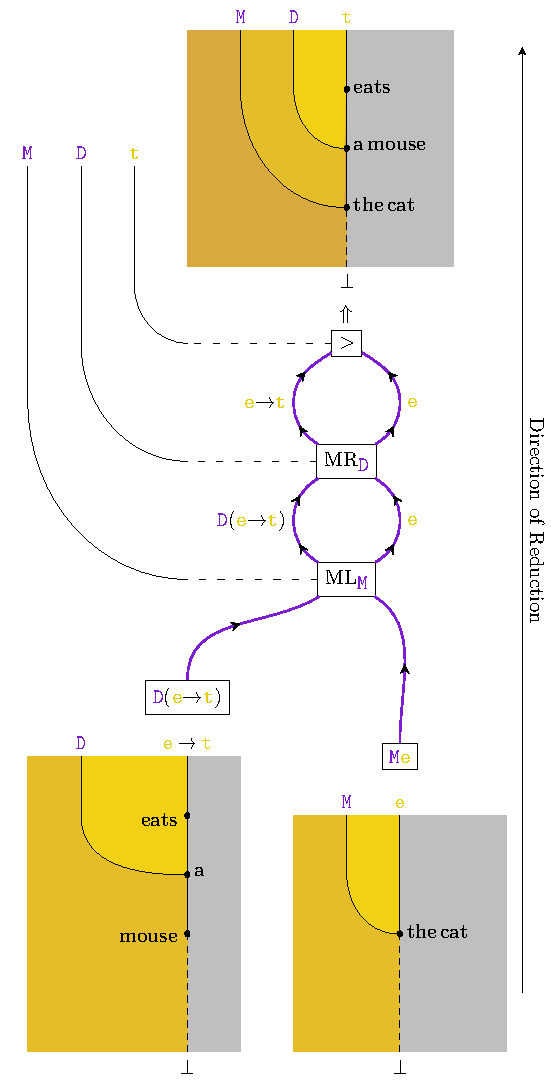
\includegraphics[width=.45\textwidth]{parsing-diagram}
	\caption{Representation of a parsing diagram for the sentence
		\emph{the cat eats a mouse}.
		See Figure \ref{fig:tree-box} for translation in a parse tree.}
	\label{fig:parsing-diagram}
\end{wrapfigure}

We can now return to the proof of the main result of this section:
\begin{proof}[Proof of Theorem \ref{thm:ptime-denot}]
	From Theorem \ref{thm:ptime-parse} we can retrieve a
	semantic parse tree from a sentence in polynomial time in the input.
	Lemma \ref{lem:quad-tree} states that we have a polynomial number of
	combinator denotations to apply, all done in polynomial time by hypothesis.
	We have already seen that given a denotation, handling all effects and
	reducing effect handling to normal forms can be done in polynomial time.
	The sequencing of these steps yields a polynomial-time algorithm in the
	length of the input sentence.
\end{proof}

While we have gone the hypothesis that we have a CFG for our language,
any type of polynomial-time structure could work, as long as it is more
expressive than a CFG.

The \emph{polynomial time combinators} assumption in Theorem
\ref{thm:ptime-denot} is not a complex assumption, this is for example true for
denotations based on lambda-calculus, with function application being linear in
the number of uses of variables in the function term, which in turn is linear
in the number of terms used to construct the function term and thus of words,
and the different \fmap{} being in polynomial time for the same reason.
This would also be true for denotations inspired by machine learning for
example.

\subsection{Diagrammatical Parsing}
When considering \cite{coeckeMathematicalFoundationsCompositional2010}
way of using string diagrams for syntactic parsing/reductions, we can see
string diagrams as (yet) another way of writing our parsing rules.
They are an expanded rewriting of labelled parsing trees\footnote{Point of view
	which connects this formalism nicely to the one of
	\cite{senturiaAlgebraicStructureMorphosyntax2025}, preserving all their
	results inside our theory.} presented in
\cite{bumfordEffectdrivenInterpretationFunctors2025}, .
In our typed category, we can see our combinators as natural transformations
($2$-cells): then we can see the different sets of combinators as different
arity natural transformations.
Combinators $>$, $\combML_{\f{F}}$ and $\combJ_{\f{F}}$ are represented in
Figure \ref{fig:combinator-sd}.
The coloring of the regions is purely for artistic rendition and will not be
used for larger diagrams.

\begin{wrapfigure}{r}{.45\textwidth}
	\centering
	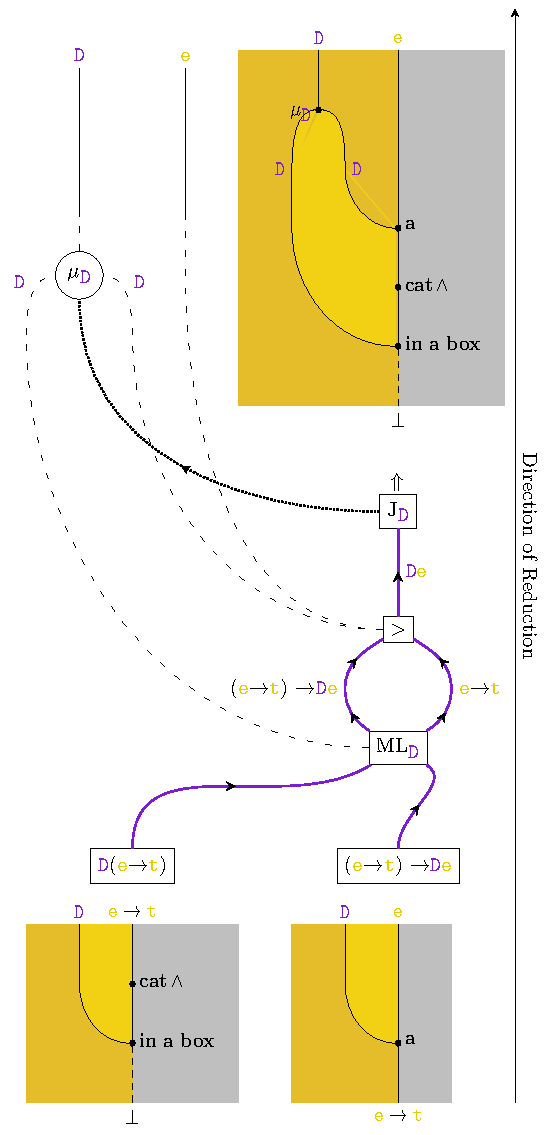
\includegraphics[width=.45\textwidth]{parsing-diagram2.pdf}
	\caption{Example of a parsing diagram for the phrase
		\emph{a cat in a box}, presenting the integration of unary combinators
		inside the connector line. See Figure \ref{fig:tree-box} for translation in
		a parse tree.}
	\label{fig:parsing-diagram2}
\end{wrapfigure}
Understanding the diagrams could be thinking of them on an orthogonal plane to
the ones of Section \ref{sec:nondet}: we could use the syntactic version of the
diagrams to model our parsing, according to the rules in Figure
\ref{fig:combination-cfg}, and then combine the diagrams as shown in Figure
\ref{fig:parsing-diagram}, which highlights the \emph{orthogonal} components.
In this diagram we exactly see the sequence of combinations play out on the
types of the words, and thus we also see what exact \emph{stitch} would
be needed to construct the effect diagram.
Here we talk about \emph{stitches} because, in a sense, we use $2$-cells
to do braiding-like operations on the strings, and don't actually allow for
braiding inside the diagrammatic computation, leading to the intervention of
outside tools (combinators) which one might see as \emph{knitting needles}.
To better understand what happens in those parsing diagrams, Figure
\ref{fig:parsing-trees} provides the translations in labelled trees of the
parsing diagrams of Figures \ref{fig:parsing-diagram},
\ref{fig:parsing-diagram2} and \ref{fig:3dparsing-diagram}.


For the combinators $\combJ$, $\combDN$ and $\combC$, which are applied to
reduce the number of effects inside a denotation, it might seem less obvious
how to include them.
Applying them to the actual \emph{parsing} part of the diagram is done
in the exact same way as in the CFG: we just add them where needed, and they
will appear in the resulting denotation as a form of forced handling, in a
sense, as shown in the result of Figure \ref{fig:parsing-diagram2}.
It is interesting to note that the resulting diagram representing
the sentence can visually be found in the connection strings that arise from
the combinators.

\smallskip

Categorically, we start from a meaning category $\mC$, our typing category, and
take it as our grammatical category.
This is a form of extension on the monoidal version by
\cite{coeckeMathematicalFoundationsCompositional2010} and
\cite{toumiHigherOrderDisCoCatPeirceLambekMontague2023}, as it is seemingly a
typed version, where we change the pregroup category for the typing category,
taken with a product for representation of the English grammar representation,
to accommodate for syntactic typing on top of semantic typing if it does not
already encompass it.
We have a first plane of string diagrams in the category
$\mC$ - our string diagrams for effect handling, as in Section
\ref{sec:nondet} - and the second \emph{orthogonal} plane of string diagrams
on a larger category, with formal endofunctors labelled by the types in our
typing category $\bar{\mC}$ and formal natural transformations for the
combinators defined in Figures \ref{fig:combination-cfg} and
\ref{fig:combinator-denotations}.
The category in which we consider the second-axis string diagrams does not have
a meaning in our compositional semantics theory, and to be more precise, we
should talk about $1$-cells and $2$-cells instead of endofunctors and natural
transformations, to keep in the idea that this is really just a diagrammatic
way of computing and presenting the operations that are put to work during
semantic parsing.

\begin{wrapfigure}{r}{.45\textwidth}
	\centering
	\begin{tikzpicture}
		\node (fig) at (0, 0) {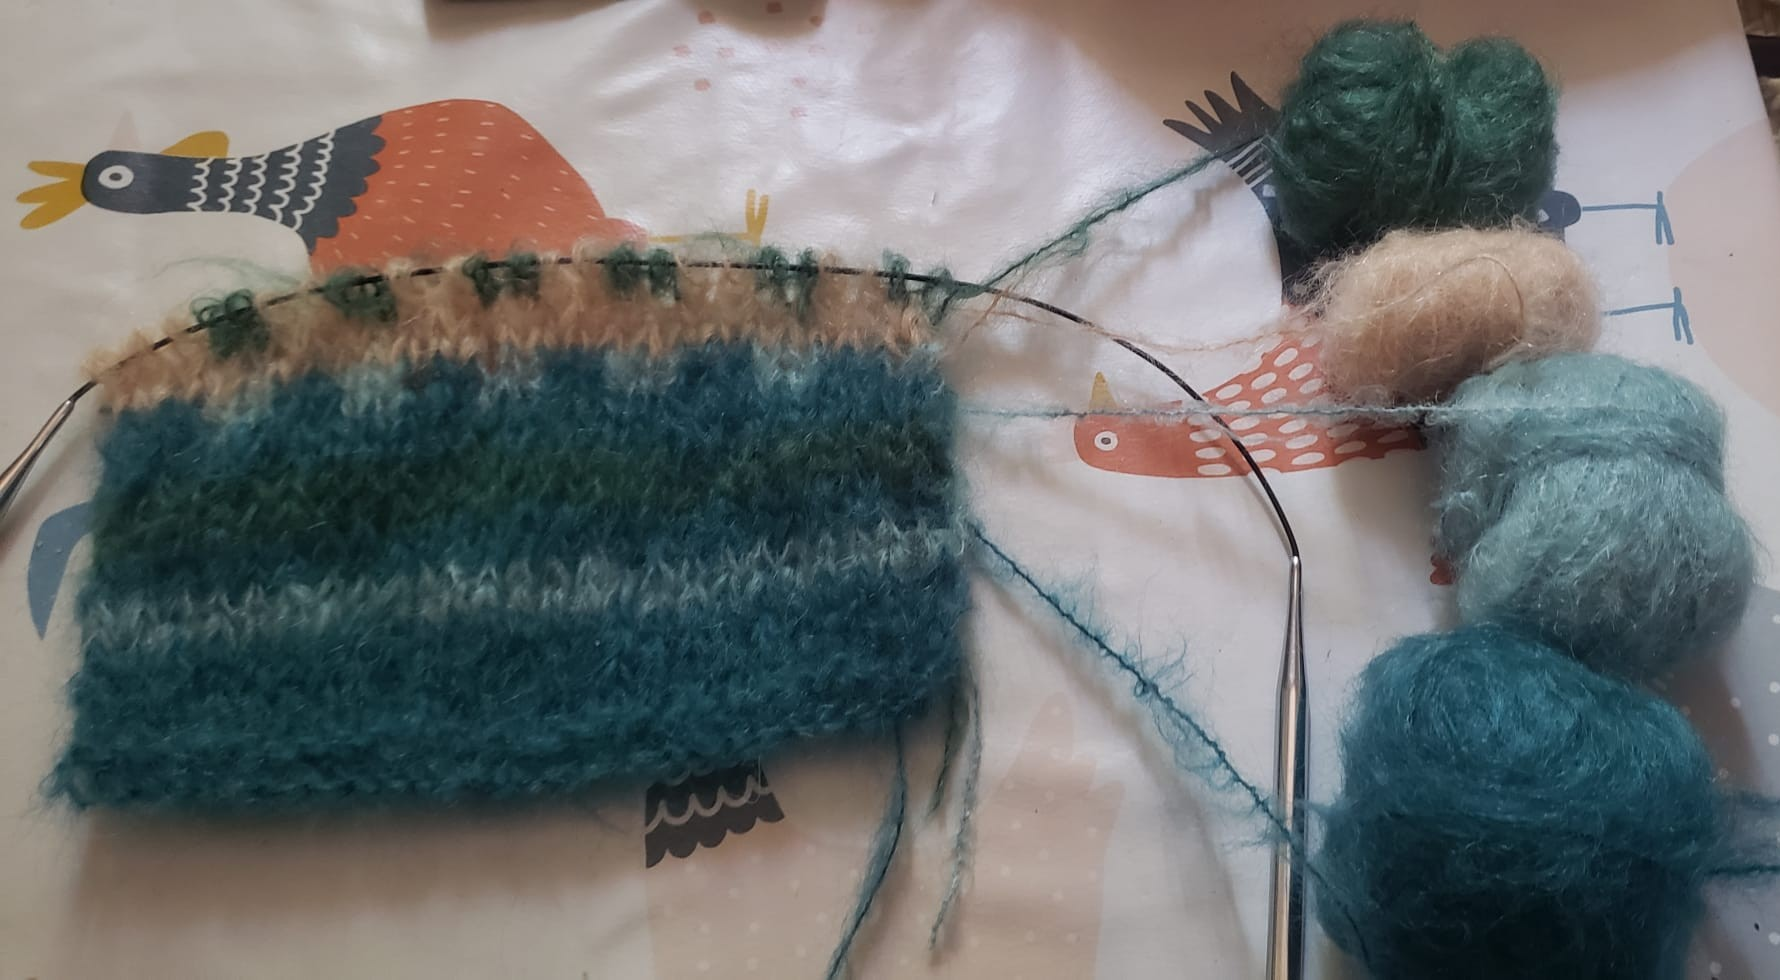
\includegraphics[width=.4\textwidth]{knitting-example}};
		\draw[->] ($(fig.south west) + (-.1, -.1)$) -- node[anchor=east] {\rotatebox{90}{Direction of Reduction}} ($(fig.north west) + (-.1, .1)$);
	\end{tikzpicture}
	\caption{Example of a \emph{Jacquard} knitwork. Photography and work courtesy
		of the author's mother.}
	\label{fig:knitting-example}
\end{wrapfigure}

The main theoretical reason why this point of view of diagrammatic parsing is
useful will be clear when looking at the rewriting rules and the normal forms
they induce, because, as stated in Theorem \ref{thm:norm}, string
diagrams make it easy to compute normal forms when provided with a confluent
reduction system.
However, the just as useful graphical interpretation of string diagrams as
easy to read expanded labelled parsing trees.
Using orthogonal planes to visualise this interpretation cannot be well
presented in a 3D space, and even less so on a page, so we suggest an
interpretation based on actual strings:
Suppose you're knitting a rainbow scarf.
You have multiple threads (the different words) of the different colours (their
types and effects) you're using to knit the scarf.
When you decide to change the color you take the different threads you have
been using, and mix them up.

\begin{wrapfigure}[22]{l}{.5\textwidth}
	\centering
	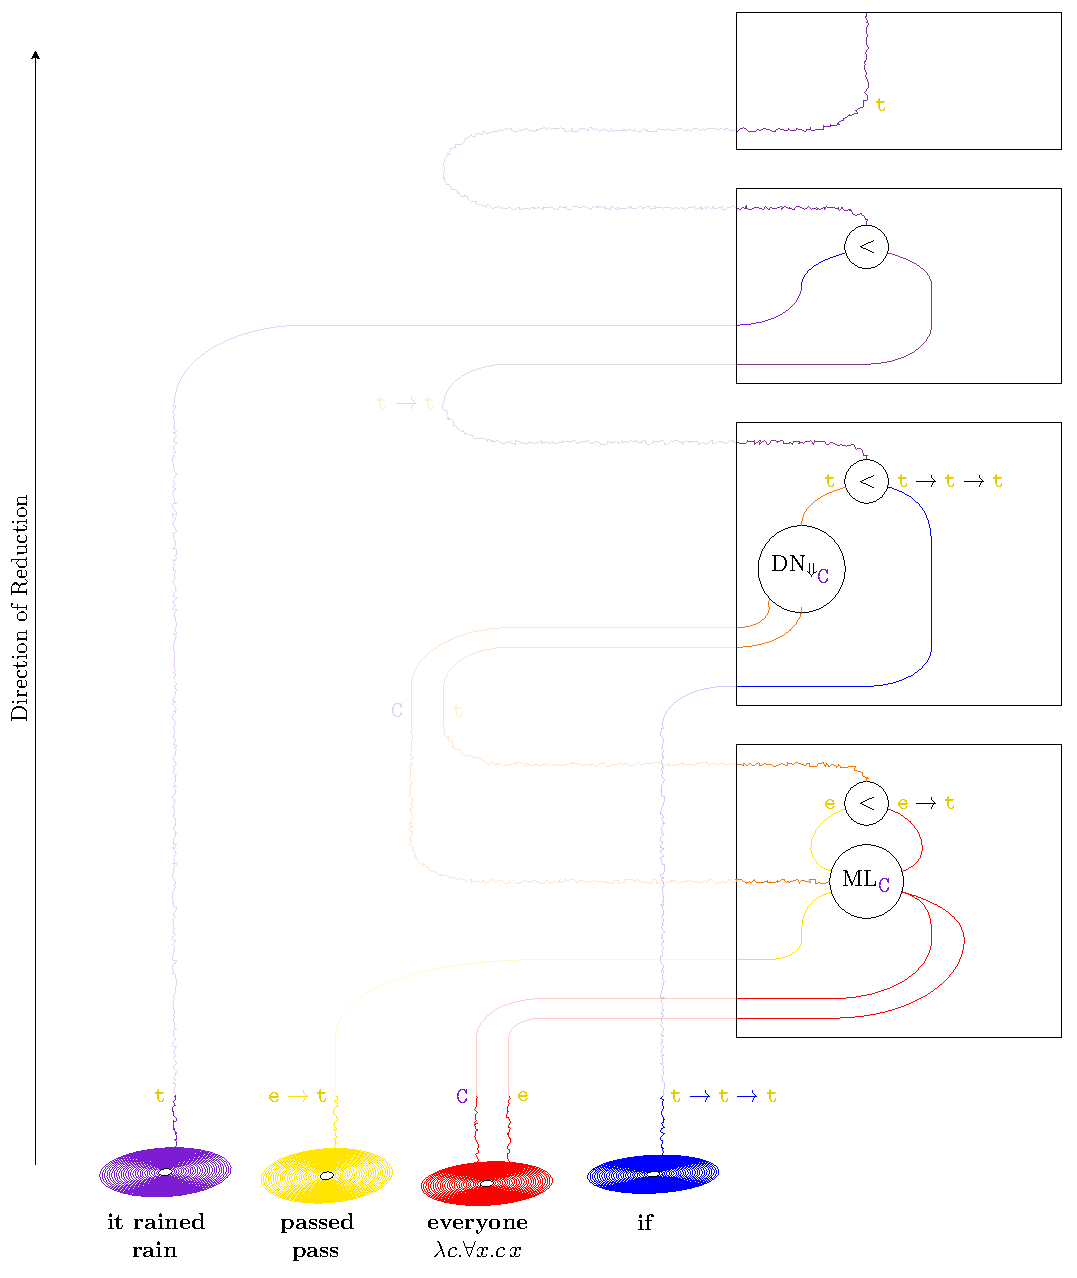
\includegraphics[width=.5\textwidth]{3d-parsing-diagram}
	\caption{Knitting-like representation of the diagrammatic parsing of a sentence. See Figure \ref{fig:tree-rain} for the translation in a parse tree}
	\label{fig:3dparsing-diagram}
\end{wrapfigure}

You can create a new colour\footnote{This is not how wool works, but
	if one can also imagine a pointillist-like way of drawing using multiple
	coloured lines that superimpose on each other, or a marching band's multiple
	instruments playing either in harmony or in disharmony and changing that
	during a score.} thread from two (that's the base combinators).
Creating a thicker one from two of the same colour is the result of the
applicative mode and the monadic join.
$\fmap$ puts aside a thread until a later step, the monadic unit adds a new
thread to the pattern, and the co-unit and closure operators cut a thread which
will no longer be used.
Changing a thread by cutting it and making a knot at another point is what the
eject combinators do.

This more tangible representation can be seen in Figure
\ref{fig:3dparsing-diagram}.
The sections in the rectangle represent what happen when considering our
combination step as implementing patterns inside a knitwork, as seen in Figure
\ref{fig:knitting-example}.
The different patterns provide, in order, a visual representation of the
different ways one can combine two strings, i.e., two types and thus two
denotations.
The sections outside of the rectangle are the strings of yarn not currently
being used to make a pattern.

\subsection{Rewriting Rules}
\label{subsec:rewrite}
In this section we study reductions for our diagrams that allows us
to improve our time complexity by reducing the size of the grammar.
This is done by looking at equations on sequences of combinators.
In the worst case, there is no improvement in big o notation in the size of the
sentence, but there is no loss.

\noindent Consider the case where we have the two arguments of our parsing step of
type $\f{F}\tau$ and $\f{G}\tau'$.
In that case we could either get a result with effects $\f{F}\f{G}$ or
with effects $\f{G}\f{F}$.
If those effects happen to be equal, which trivially will be the case when one
of the effects is external (the plural or islands functors for example), the
order of application does not matter and we choose to get the effect on the
left side of the combinator first: $\combML_{\f{F}}\combMR_{\f{G}}$ over
$\combMR_{\f{F}}\combML_{\f{F}}$.

\noindent There are sequence of modes that clearly encompass other ones
the grammar notation for ease of explanation.
One should not use the unit of a functor after using $\combML$ or $\combMR$, as
that adds void semantics.
Same things can be said for certain other derivations containing the lowering
and co-unit combinators since they could in theory be applied at many points
inside the derivation.

\noindent We use $\combDN$ when we have not used any of the following, in all
derivations:
\let\mcolsep=\multicolsep
\setlength{\multicolsep}{.4\mcolsep}
\begin{multicols}{2}
	\begin{itemize}
		\item $m_{\f{F}}, \combDN, m_{\f{F}}$ where
		      $m \in \{\combMR, \combML\}$
		\item $\combML_{\f{F}}, \combDN, \combMR_{\f{F}}$
		\item $\combA_{\f{F}}, \combDN, \combMR_{\f{F}}$
		\item $\combML_{\f{F}}, \combDN, \combA_{\f{F}}$
		\item $\combC$
	\end{itemize}
\end{multicols}
\noindent We use $\combJ$ if we have not used any of the following,
for $j \in \{\epsilon, \combJ_{\f{F}}\}$
\begin{multicols}{2}
	\begin{itemize}
		\item $\left\{m_{\f{F}}, j, m_{\f{F}}\right\}$ where
		      $m \in \{\combMR, \combML\}$
		\item $\combML_{\f{F}}, j, \combMR_{\f{f}}$
		\item $\combA_{\f{F}}, j, \combMR_{\f{F}}$,
		\item $\combML_{\f{F}}, j, \combA_{\f{F}}$
		\item $k, \combC$ for $k \in \{\epsilon, \combA_{\f{F}}\}$
		\item If $\f{F}$ is commutative as a monad:
		      \begin{itemize}
			      \item $\combMR_{\f{F}}, \combA_{\f{F}}$
			      \item $\combA_{\f{F}}, \combML_{\f{F}}$
			      \item $\combMR_{\f{F}}, j, \combML_{\f{F}}$
			      \item $\combA_{\f{F}}, j, \combA_{\f{F}}$
		      \end{itemize}
	\end{itemize}
\end{multicols}

\begin{theorem}
	The rules proposed above yield equivalent results.
\end{theorem}
\begin{proof}
	The rules about not using combinators $\combUL$ and $\combUR$ come from the
	notion of handling and granting termination and decidability to our system.
	The rules about adding $\combJ$ and $\combDN$ after moving two of the same
	effect from the same side (i.e. $\combML \combML$ or $\combMR\combMR$) are
	normalization along Theorem \ref{thm:isotopy}: the only reason to keep two of
	the same effects and not join them is to at some point	have something get in
	between the two.
	Joining and closure should then be done at earliest point in parsing where it
	can be done, and that is equivalent to later points because of Theorem
	\ref{thm:isotopy}.
	The last set of rules follows from the following: we should not use $\combJ
		\combML \combMR$ instead of $\combA$, as those are equivalent because of the
	equation defining them.
	The same thing goes for the other two, as we should use the units of monads
	over applicative rules and \fmap.
\end{proof}

The reductions described above amount to equational reductions for the string
diagrams, as they are equivalent to specific sequences of $2$-cells.
This leads to the same algorithms developed in Section \ref{sec:nondet} being
usable here: we just have a new improved version of Theorem
\ref{thm:confluence}: computing two different normal forms along the
tensor product of our reduction schemes, which amounts to computing a larger
normal form.
Theorem \ref{thm:norm} still stands with the improved system and thus, proving
two parses are equal can be done in polynomial time.
Moreover, considering the possible normal forms of syntactic reductions
or denotational reductions adds ways to reduce our diagrams to normal forms.
